% OpenSmFe manuscript template. Numbers are filled in from the database by code/06_manuscript.py.
% Placeholders are double angle brackets around a key name. Do not type numbers into this file; edit the script instead.
\documentclass[10pt,twocolumn,letterpaper]{article}
\usepackage[T1]{fontenc}
\usepackage{mathptmx}
\usepackage[top=0.75in,bottom=0.8in,left=0.7in,right=0.7in,columnsep=0.25in]{geometry}
\usepackage{amsmath,amssymb,graphicx,booktabs,xcolor,array}
\usepackage[labelsep=period,font=small,justification=justified,singlelinecheck=false]{caption}
\usepackage[hidelinks]{hyperref}
\captionsetup[figure]{name=FIG.}
\captionsetup[table]{name=TABLE,justification=centering}
\renewcommand{\thetable}{\Roman{table}}
\renewcommand{\thesection}{\Roman{section}}
\renewcommand{\thesubsection}{\Alph{subsection}}
\makeatletter
\renewcommand\section{\@startsection{section}{1}{\z@}{2.2ex plus .5ex}{1.2ex}{\centering\normalfont\small\bfseries\MakeUppercase}}
\renewcommand\subsection{\@startsection{subsection}{2}{\z@}{1.8ex plus .4ex}{1ex}{\centering\normalfont\small\bfseries}}
\renewcommand\@seccntformat[1]{\csname the#1\endcsname.\quad}
\renewcommand\p@subsection{\thesection\,}
\renewcommand\@biblabel[1]{[#1]}
\makeatother
\setlength{\parindent}{1em}
\setlength{\parskip}{0pt}
\newcommand{\SmFeN}{Sm$_2$Fe$_{17}$N$_3$}
\newcommand{\SmFe}{Sm$_2$Fe$_{17}$}
\newcommand{\kAm}{kA\,m$^{-1}$}
\newcommand{\kJm}{kJ\,m$^{-3}$}
\newcommand{\phead}[1]{\emph{#1}---}

\begin{document}
\twocolumn[
\begin{@twocolumnfalse}
\begin{center}
{\large\bfseries OpenSmFe: An Open, Processing-Aware and Comparability-Graded Database\\ of Samarium--Iron(--Nitrogen) Permanent-Magnet Properties\par}
\vspace{2.2ex}
{\normalsize Joshua Chukwuemeka Ejeka$^{*}$\par}
\vspace{0.6ex}
{\small\itshape Independent Researcher\par}
\vspace{0.4ex}
{\small (Dated: \today)\par}
\vspace{1.8ex}
\begin{minipage}{0.82\textwidth}
\small
\setlength{\parindent}{1em}
Samarium--iron--nitride (\SmFeN) is a leading rare-earth-lean candidate for high-performance permanent magnets, but its published properties are difficult to compare. The nitride decomposes below conventional sintering temperatures, so reported values come from loose powders, aligned powders, bonded magnets and low-temperature consolidated compacts, measured under conditions that papers often leave unstated. Text-mined materials databases now reach tens of thousands of entries, but they record a value without the processing route, sample form and measurement conditions that determine what the value means. We describe OpenSmFe, an open database in which every value is stored as published, converted to SI units, linked to a verbatim evidence sentence, and assigned an explicit A/B/C comparability grade with machine-readable reasons. The schema separates samples (composition, alloy route, milling, melt spinning, annealing, nitriding, consolidation, phase outcome and sample form) from measurements. We apply it to a seed release of 21 author-verified values from 14 samples in 6 open-access papers. No value attains the highest grade. The measurement temperature is unstated for 16 of the 19 values other than Curie temperatures, and the coercivity definition is unstated for 8 of 11 coercivities. The workflow also exposed an internal inconsistency in one source. It caught 1 misattributed and 3 paraphrased evidence statements in the AI-assisted first-draft extraction, all corrected before release. We propose a minimum reporting set for Sm--Fe--N magnet studies and release the data and code under open licenses.
\end{minipage}
\end{center}
\vspace{2.5ex}
\end{@twocolumnfalse}
]
{\renewcommand{\thefootnote}{\fnsymbol{footnote}}\footnotetext[1]{jejeka@uwyo.edu}}

\section{Introduction}

Permanent magnets convert between electrical and mechanical energy in electric-vehicle traction motors, wind-turbine generators and a wide range of industrial and defense systems~\cite{gutfleisch2011,coey2020}. The highest-performance commercial magnets are based on Nd$_2$Fe$_{14}$B. Their supply chain is geographically concentrated, and the U.S. Department of Energy lists the rare-earth elements used in them among critical materials~\cite{doe2023}. Alternatives that use less of the most supply-constrained rare earths, or that tolerate higher operating temperatures, are therefore of both scientific and strategic interest~\cite{coey2020}.

\SmFeN\ is one of the most studied such alternatives. Interstitial nitrogenation of the \SmFe\ intermetallic converts a compound with planar anisotropy and a low Curie temperature into one with strong uniaxial anisotropy and a substantially higher Curie temperature~\cite{coeysun1990}. The nitride is reported to combine a saturation polarization of about 1.54~T, an anisotropy field of about 14~T and a Curie temperature near 475~$^\circ$C~\cite{xu2024}, compared with about 585~K for Nd$_2$Fe$_{14}$B~\cite{saito2024}. These intrinsic properties make it attractive for magnets that must keep their performance at elevated temperature.

Turning these intrinsic properties into a magnet is the difficulty. \SmFeN\ decomposes into SmN and $\alpha$-Fe at elevated temperature~\cite{saito2024}, so the liquid-phase sintering used for Nd--Fe--B is not available. Practical magnets are instead made by bonding powders in a polymer or metal binder, or by consolidating them at reduced temperature: spark-plasma sintering~\cite{saito2024}, hot pressing with a low-melting alloy binder~\cite{zheng2022}, or sintering under strictly controlled oxygen~\cite{soda2016}. The starting powders themselves are produced by several distinct routes. These include strip casting followed by nitriding and milling~\cite{liang2023}, calcium reduction--diffusion from oxide precursors~\cite{saito2024,zheng2020,okada2017}, and thermal-plasma synthesis of metastable TbCu$_7$-type particles~\cite{hirayama2025}. Coercivity in these materials is an extrinsic property governed by microstructure, particle size and surface condition~\cite{kronmuller2003}. The processing route is therefore not incidental metadata: it largely determines the measured result.

Comparing published results is correspondingly difficult. Values are reported in CGS and SI units. Magnetization is given per unit mass (emu\,g$^{-1}$) or as a polarization (T or kG), and only the latter can be compared directly with a bulk magnet. ``Coercivity'' may denote the intrinsic coercivity $H_{cj}$ or the normal coercivity $H_{cb}$, often without saying which. Coercivity depends strongly on temperature~\cite{xu2024}, so an unstated measurement temperature leaves a value ambiguous. For bulk magnets, standardized hysteresigraph procedures exist~\cite{iec604045,astma977}. Most powder studies use open-circuit magnetometry, where sample shape and demagnetization correction matter and are not always reported~\cite{coey2010}.

Materials-data infrastructure has grown rapidly. Rule-based and machine-learning text mining, exemplified by ChemDataExtractor~\cite{swain2016,mavracic2021}, has produced auto-generated databases such as one of Curie and N\'eel temperatures~\cite{court2018}. Large language models now extract properties at larger scale and with competitive precision~\cite{polak2024}. The Northeast Materials Database (NEMAD) applies them to about 67,000 magnetic materials, including coercivity and remanence~\cite{itani2025}. Text mining has also been applied to synthesis procedures~\cite{kim2017}, and computed-property databases cover intrinsic quantities across hundreds of thousands of compounds~\cite{jain2013}. These resources are valuable for discovery and breadth. For an extrinsic quantity such as coercivity, however, a compound--value pair is not sufficient: two values for ``\SmFeN'' can differ by more than an order of magnitude because one was measured on an aligned micrometre powder and the other on a consolidated compact. What is missing is a record that keeps the processing context and measurement conditions attached to each value, states openly when they are absent, and lets a reader judge which values may be compared. Keeping that context and provenance attached is also what makes such data findable, accessible, interoperable and reusable~\cite{wilkinson2016}.

This paper describes OpenSmFe, a database built to supply that record for the Sm--Fe(--N) family. Its contributions are:
(i)~a schema that separates samples, with their composition and full processing route, from individual measurements;
(ii)~an explicit, rule-based comparability grade with machine-readable reasons on every value;
(iii)~an evidence-linked curation workflow in which every value carries a verbatim source sentence and passes automated containment and physical-consistency checks before author verification;
(iv)~a seed release, analyzed here, that quantifies how often the information needed for comparison is missing; and
(v)~a proposed minimum reporting set for Sm--Fe--N magnet studies.
Sections~\ref{sec:design} and~\ref{sec:workflow} describe the design and workflow, Sec.~\ref{sec:results} the seed release, and Sec.~\ref{sec:discussion} its implications and limitations.

\section{Database design}\label{sec:design}

\subsection{Scope and unit of record}

Version 0.1 covers compounds based on the \SmFe\ structure (the rhombohedral Th$_2$Zn$_{17}$ and hexagonal Th$_2$Ni$_{17}$ types, ``2:17'') and the disordered TbCu$_7$-type phase (``1:7''), nitrided or not, including substituted variants. The ThMn$_{12}$-type SmFe$_{12}$ family is deferred to a later version. Soft/hard composites, hybrid Nd--Fe--B/Sm--Fe--N magnets and fluorinated or carbided interstitial compounds are excluded. Only \emph{primary} values are recorded: values a paper reports for its own samples. Values quoted from earlier work, including all values in review articles, are not entered; reviews are used only to locate primary sources.

The unit of record is a \emph{measurement}: one property of one sample at one measurement temperature. Measurements reference a \emph{sample}, which references a \emph{source}. Each table is released as comma-separated values, together with a flat join for spreadsheet users.

\subsection{Sample schema}

A sample is one distinct material state described in one paper. Its fields record the nominal composition; the family (2:17 or 1:7); whether it was nitrided; the alloy or powder route (for example arc melting, strip casting, reduction--diffusion, spray pyrolysis, thermal plasma or commercial powder); milling; melt spinning (wheel speed); annealing (temperature, time and atmosphere); nitriding (temperature, time and gas); and consolidation (bonding, sintering, hot pressing or alignment, with conditions). It also records the reported phase outcome, the sample form (powder, aligned powder, powder aligned in resin, sintered or bonded bulk, ribbon or film), whether the sample was magnetically aligned, and the mean particle size. Fields are recorded in the paper's own terms. Where a paper does not report a field, the record says so explicitly (``not stated in abstract'') rather than leaving a blank that could be read as zero or as an omission by the curator.

\subsection{Measurement schema and unit harmonization}

Each measurement stores the property, the value and unit exactly as printed, a converted SI value, the measurement temperature and its status (stated, implied but unconfirmed, not stated, or not applicable), the instrument when stated, the verbatim evidence sentence and its location in the paper, the comparability grade with reasons, and the verification status.

The properties are the intrinsic coercivity $H_{cj}$; the normal coercivity $H_{cb}$; a coercivity whose definition the paper does not give, $H_c$; the remanence $B_r$ (volume basis) or remanent magnetization $\sigma_r$ (mass basis); the saturation magnetization; the maximum energy product $(BH)_{\max}$; and the Curie temperature $T_C$. Coercivities are converted to \kAm,
\begin{equation}
H\,[\text{kA\,m}^{-1}] = \frac{10^3}{4\pi}\,H\,[\text{kOe}] = \frac{\mu_0 H\,[\text{T}]}{\mu_0}\times10^{-3},
\label{eq:hc}
\end{equation}
so that 1~kOe $=79.58$~\kAm. Energy products are converted as $(BH)_{\max}[\text{kJ\,m}^{-3}]=(10^2/4\pi)\,(BH)_{\max}[\text{MGOe}]$, so that 1~MGOe $=7.958$~\kJm. Polarizations in kG are converted to tesla, and Curie temperatures to kelvin.

Magnetization is kept on its published basis. A specific magnetization $\sigma$ (A\,m$^2$\,kg$^{-1}$, numerically equal to emu\,g$^{-1}$) corresponds to a polarization
\begin{equation}
J = \mu_0 \rho\, \sigma ,
\label{eq:basis}
\end{equation}
which requires the density $\rho$ of the measured body. Powders and bonded or partially densified magnets are rarely reported with a density, so OpenSmFe does not perform this conversion. Mass-basis values reported for bulk magnets are flagged instead (Sec.~\ref{sec:grade}).

\subsection{Comparability grade}\label{sec:grade}

Every measurement receives a grade computed by fixed rules from its own fields (Table~\ref{tab:grade}). A \emph{hard} reason makes a value not directly comparable with ambient-temperature data. A \emph{soft} reason leaves it comparable only with care. The grade is
\begin{equation}
g=\begin{cases}
\text{C} & \text{if } R_{\text{hard}}\neq\varnothing,\\
\text{B} & \text{if } R_{\text{hard}}=\varnothing,\ R_{\text{soft}}\neq\varnothing,\\
\text{A} & \text{otherwise,}
\end{cases}
\end{equation}
where $R_{\text{hard}}$ and $R_{\text{soft}}$ are the sets of applicable reasons, all of which are stored with the row. Room temperature is defined as 290--305~K when stated. An unstated temperature is not assumed to be ambient, because doing so would raise the apparent quality of the record without information to support it. Grades are recomputed on every build. When a verifier records the measurement temperature or coercivity definition from a paper's methods section, the affected rows re-grade automatically.

\begin{table}[t]
\caption{Comparability rules. A value is graded C if any hard reason applies, B if only soft reasons apply, and A otherwise.}
\label{tab:grade}
\small
\begin{tabular}{@{}p{0.70\columnwidth}l@{}}
\toprule
Reason & Class \\
\midrule
Measured outside 290--305 K (e.g.\ 10 K) & hard \\
Measurement temperature not stated & soft \\
Room temperature implied but not confirmed & soft \\
Coercivity definition ($H_{cj}$ or $H_{cb}$) not stated & soft \\
Mass-basis magnetization reported for a bulk magnet & soft \\
$(BH)_{\max}$ of a loose powder (depends on assumed packing) & soft \\
Sample form not confirmed & soft \\
Value reported inconsistently within the source & soft \\
$T_C$ approximate, or possibly quoted rather than measured & soft \\
\bottomrule
\end{tabular}
\end{table}

\subsection{Consistency checks}

Each build runs automated checks and writes a quality report. Converted values must fall within physically plausible ranges for the family. Each published number must appear verbatim in its own evidence sentence; this check catches transcription errors and evidence attached to the wrong statement. Within a sample, the energy product must satisfy the ideal square-loop bound
\begin{equation}
(BH)_{\max} \le \frac{B_r^2}{4\mu_0},
\label{eq:bound}
\end{equation}
and remanent magnetization may not exceed saturation magnetization. Duplicate identifiers and missing required sample fields are also reported. A release is blocked while any check fails or any field carries an unresolved verification marker.

\section{Curation workflow}\label{sec:workflow}

\subsection{Discovery and screening}

Candidate papers were identified by a title query of the Directory of Open Access Journals~\cite{doaj} for ``\SmFeN'', ``Sm-Fe-N'' or ``\SmFe'', supplemented by targeted searches for open-access journals. In total 24 records were screened for v0.1:
\begin{itemize}\setlength{\itemsep}{0pt}
\item 6 were extracted;
\item 10 are queued for full-text extraction, because their publishers block automated reading;
\item 3 are queued for partial extraction of in-scope reference samples only;
\item 2 are reviews, used only to locate primary sources;
\item 1 is deferred to the SmFe$_{12}$ scope;
\item 2 were excluded.
\end{itemize}
Each decision and its reason are released with the data, so the screening can be audited and extended.

\subsection{Extraction}

A first draft of each extraction was produced with an AI assistant reading the publisher's web page. Each value was recorded with its verbatim evidence sentence (at most one sentence) and its location (abstract, section, table or figure caption). For 3 sources the full text was read. For 3 sources only the abstract could be read, because the publisher's full-text page was not accessible to automated reading; this is recorded per source. Values that appear only in plots were not digitized in v0.1.

\subsection{Verification and curation corrections}

Every first-draft extraction was checked against its source, and all corrections were logged. The curation log records 3 evidence statements that were paraphrases rather than verbatim text and were replaced. In 2 cases the verbatim text showed that a paper reports intrinsic coercivity (``iHc''), and the property was reclassified from $H_c$ to $H_{cj}$. In 1 case a correct value had been attached to a general statement instead of the sentence reporting the measurement. In 2 cases a measurement temperature had been assumed and was changed to ``not stated''. No numerical value was changed during curation. The errors were in evidence, labels and context, which is exactly what a value-only record cannot show. The author then verified all 21 values against their sources before release. Verification was recorded at the release level, as discussed in Sec.~\ref{sec:limits}.

\subsection{Reproducibility}

The database is rebuilt from the raw extraction tables by a sequence of scripts that register the inputs with SHA-256 fingerprints, harmonize units, assign grades, apply the verification log, run the checks, and draw the figures. A rebuild from a clean copy reproduces the released tables byte for byte. The tables, figures and every number in this manuscript are generated from the released files~\cite{opensmfe}.

\section{The seed release}\label{sec:results}

\subsection{Composition}

Version 0.1 contains 21 measurements of 14 samples from 6 papers published between 2020 and 2025 (Table~\ref{tab:sources}). 13 samples belong to the 2:17 family and 1 to the TbCu$_7$-type family, and 13 of the 14 are nitrided. The measurements comprise 11 coercivities (3 explicitly intrinsic), 5 mass-basis remanent magnetizations, 1 volume-basis remanence, 2 energy products and 2 Curie temperatures. All 21 are listed in Table~\ref{tab:meas}. The release is deliberately small: it establishes and tests the schema, grading and workflow before the database is expanded.


\begin{table*}[t]
\caption{Sources in OpenSmFe v0.1. ``Text'' indicates whether values were extracted from the full text or from the abstract only.}
\label{tab:sources}
\small
\begin{tabular}{@{}lllp{0.22\textwidth}cc@{}}
\toprule
Source & Year & Powder or alloy route & Sample forms & Values & Text \\
\midrule
Saito~\cite{saito2024} & 2024 & reduction-diffusion & aligned powder, powder, sintered bulk & 11 & full \\
Liang \textit{et al.}~\cite{liang2023} & 2023 & strip casting & powder & 3 & abstract \\
Zheng \textit{et al.}~\cite{zheng2020} & 2020 & ultrasonic spray pyrolysis + H2 reduction precursor & powder & 1 & abstract \\
Ye \textit{et al.}~\cite{ye2024} & 2024 & commercial Sm-Fe-N powder & powder & 1 & abstract \\
Hirayama \textit{et al.}~\cite{hirayama2025} & 2025 & induction thermal plasma & aligned powder in resin & 2 & full \\
Zheng \textit{et al.}~\cite{zheng2022} & 2022 & commercial Sm$_{2}$Fe$_{17}$N$_{3}$ powder & bonded bulk & 3 & full \\
\bottomrule
\end{tabular}
\end{table*}

\begin{table*}[t]
\caption{All measurements in OpenSmFe v0.1 (each verified against its source). Values as published and converted to SI units; $T$ is the measurement temperature in kelvin (n.s., not stated). Grades follow Table~\ref{tab:grade}; reasons for each grade, evidence sentences and full processing fields are in the released files.}
\label{tab:meas}
\footnotesize
\begin{tabular}{@{}llllllc@{}}
\toprule
Sample & Description & Property & As published & SI & $T$ (K) & Grade \\
\midrule
SAITO2024-a & Sm$_{2}$Fe$_{17}$N$_{3}$ powder (unaligned) & $H_c$ & 12.4 kOe & 986.8 kA\,m$^{-1}$ & n.s. & B \\
SAITO2024-a & Sm$_{2}$Fe$_{17}$N$_{3}$ powder (unaligned) & $\sigma_r$ & 75.3 emu\,g$^{-1}$ & 75.3 A\,m$^2$\,kg$^{-1}$ & n.s. & B \\
SAITO2024-b & Sm$_{2}$Fe$_{17}$N$_{3}$ powder, magnetically aligned (parallel) & $\sigma_r$ & 107 emu\,g$^{-1}$ & 107 A\,m$^2$\,kg$^{-1}$ & n.s. & B \\
SAITO2024-b & Sm$_{2}$Fe$_{17}$N$_{3}$ powder, magnetically aligned (parallel) & $H_c$ & 10.3 kOe & 819.6 kA\,m$^{-1}$ & n.s. & B \\
SAITO2024-c & SPS bulk magnet, no additive & $\sigma_r$ & 68.6 emu\,g$^{-1}$ & 68.6 A\,m$^2$\,kg$^{-1}$ & n.s. & B \\
SAITO2024-c & SPS bulk magnet, no additive & $H_c$ & 3.05 kOe & 242.7 kA\,m$^{-1}$ & n.s. & B \\
SAITO2024-d & SPS bulk magnet, 1 wt\% zinc stearate (parallel) & $\sigma_r$ & 90.6 emu\,g$^{-1}$ & 90.6 A\,m$^2$\,kg$^{-1}$ & n.s. & B \\
SAITO2024-e & SPS bulk magnet, 1 wt\% zinc stearate + 5 wt\% Zn & $\sigma_r$ & 86.8 emu\,g$^{-1}$ & 86.8 A\,m$^2$\,kg$^{-1}$ & n.s. & B \\
SAITO2024-e & SPS bulk magnet, 1 wt\% zinc stearate + 5 wt\% Zn & $H_c$ & 9.82 kOe & 781.5 kA\,m$^{-1}$ & n.s. & B \\
SAITO2024-f & Sm$_{2}$Fe$_{17}$ alloy powder & $T_C$ & 490 K & 490 K & -- & B \\
SAITO2024-g & Sm$_{2}$Fe$_{17}$N$_{3}$ powder (thermomagnetic, Fig. 3b) & $T_C$ & 740 K & 740 K & -- & B \\
LIANG2023-a & anisotropic powder, 1.3 $\mu$m & $H_{cj}$ & 17.5 kOe & 1393 kA\,m$^{-1}$ & n.s. & B \\
LIANG2023-b & anisotropic powder, 3.1 $\mu$m & $(BH)_{\max}$ & 35 MGOe & 278.5 kJ\,m$^{-3}$ & n.s. & B \\
LIANG2023-c & anisotropic powder measured at 10 K (particle size not stated in abstract) & $H_{cj}$ & 36.1 kOe & 2873 kA\,m$^{-1}$ & 10 & C \\
ZHENG2020-a & USP-HR / R-D powder, 0.616 $\mu$m & $H_c$ & 14.7 kOe & 1170 kA\,m$^{-1}$ & n.s. & B \\
YE2024-a & anisotropic Sm-Fe-N powder, designed milling & $H_c$ & 15.0 kOe & 1194 kA\,m$^{-1}$ & n.s. & B \\
HIRAYAMA2025-a & ITP nanopowder x=6.0, nitrided, aligned in resin & $H_c$ & 0.056 MA\,m$^{-1}$ & 56 kA\,m$^{-1}$ & 300 & B \\
HIRAYAMA2025-a & ITP nanopowder x=6.0, nitrided, aligned in resin & $H_c$ & 0.08 MA\,m$^{-1}$ & 80 kA\,m$^{-1}$ & 10 & C \\
ZHENG2022-a & hot-pressed magnet, 5 wt\% Ce$_{72}$Cu$_{22}$Al$_{6}$ binder & $B_r$ & 10.12 kG & 1.012 T & n.s. & B \\
ZHENG2022-a & hot-pressed magnet, 5 wt\% Ce$_{72}$Cu$_{22}$Al$_{6}$ binder & $H_{cj}$ & 5.63 kOe & 448 kA\,m$^{-1}$ & n.s. & B \\
ZHENG2022-a & hot-pressed magnet, 5 wt\% Ce$_{72}$Cu$_{22}$Al$_{6}$ binder & $(BH)_{\max}$ & 21.06 MGOe & 167.6 kJ\,m$^{-3}$ & n.s. & B \\
\bottomrule
\end{tabular}
\end{table*}

\subsection{Coercivity across processing routes}

Figure~\ref{fig:hc} places every coercivity by processing route. At ambient or unstated temperature, values range from 56~\kAm\ (0.056~MA/m) to 1393~\kAm\ (17.5~kOe), a factor of about 25. Because no cross-source value is grade A, this spread should not be read as a ranking of routes. It mixes sample forms, definitions and undocumented conditions.

Contrasts \emph{within} a single source avoid most of these differences, because the instrument, conventions and starting material are shared. Saito~\cite{saito2024} reports a coercivity of 12.4~kOe (987~\kAm) for the reduction--diffusion powder. Spark-plasma consolidation without additives lowers it to 3.05~kOe (243~\kAm, 25\% of the powder value). Adding zinc stearate and zinc powder recovers it to 9.82~kOe (782~\kAm, 79\%). The same paper reports a remanent magnetization of 107~emu\,g$^{-1}$ for magnetically aligned powder measured parallel to the alignment, against 75.3~emu\,g$^{-1}$ for unaligned powder. The consolidated magnets range from 68.6 to 90.6~emu\,g$^{-1}$. These are mass-basis values for bulk bodies and are graded B, since the corresponding polarization depends on the unreported density [Eq.~(\ref{eq:basis})].

Two sources report coercivity at both ambient and cryogenic temperature. Liang \textit{et al.}~\cite{liang2023} give an intrinsic coercivity of 1393~\kAm\ for 1.3~$\mu$m powder and 2873~\kAm\ at 10~K (a factor of 2.1), although the abstract does not say which particle size the 10~K value refers to. Hirayama \textit{et al.}~\cite{hirayama2025} report 56~\kAm\ at 300~K and 80~\kAm\ at 10~K for TbCu$_7$-type nanoparticles aligned in resin (a factor of 1.4). The 10~K values are graded C. They show how strongly an unstated measurement temperature can affect a coercivity, and why the grade separates them.

\begin{figure*}[t]
\centering
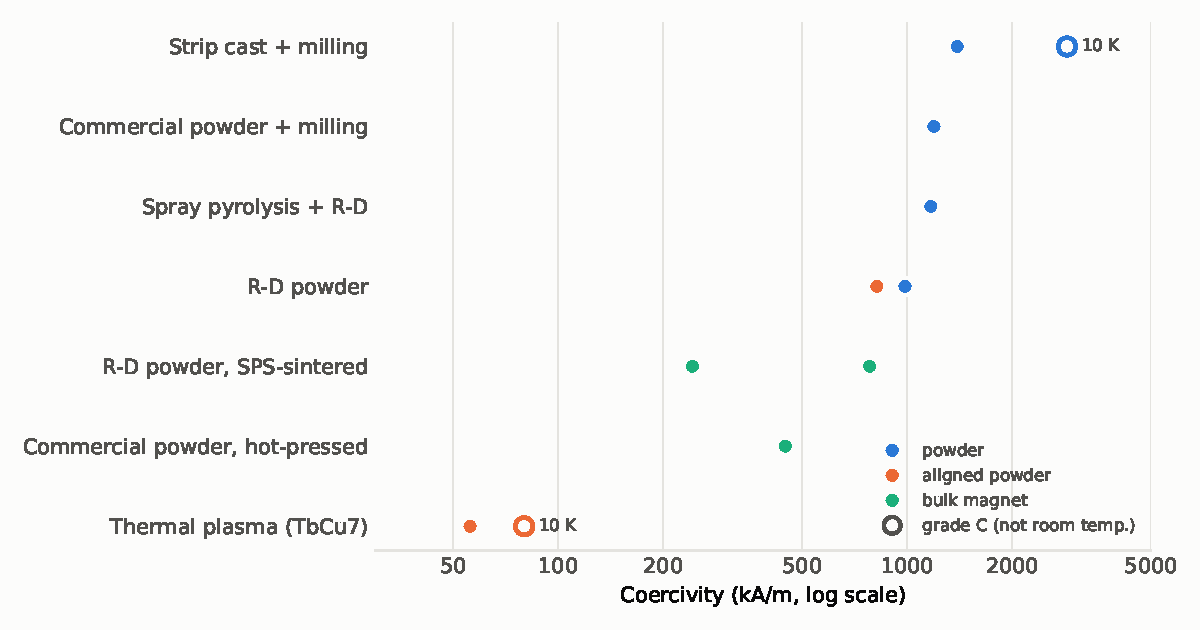
\includegraphics[width=0.80\textwidth]{fig1_coercivity_by_route.pdf}
\caption{Published coercivity of Sm--Fe(--N) samples in OpenSmFe v0.1, grouped by powder or alloy route and colored by sample form. Filled markers are values at ambient or unstated temperature (grade B); open markers are values measured at 10~K (grade C), labeled with the temperature. The horizontal axis is logarithmic. Because cross-source values differ in sample form, coercivity definition and documentation, the spread is not a ranking of routes (see text).}
\label{fig:hc}
\end{figure*}

\subsection{Energy products and physical bounds}

The square-loop bound of Eq.~(\ref{eq:bound}) gives a useful sanity check. For the intrinsic polarization of about 1.54~T~\cite{xu2024}, the ideal energy product of fully dense, perfectly aligned \SmFeN\ is $J_s^2/4\mu_0\approx$ 472~\kJm. The highest energy product in the release, 35~MGOe (278.5~\kJm) for 3.1~$\mu$m anisotropic powder~\cite{liang2023}, is 59\% of this ideal. Because it is a powder value, it depends on the packing density assumed in its evaluation and is graded B. For the hot-pressed magnet of Zheng \textit{et al.}~\cite{zheng2022}, the reported remanence of 1.012~T bounds the energy product at 203.7~\kJm. The reported 167.6~\kJm\ is 82\% of that bound, consistent with a well-squared but non-ideal loop. No value in the release violates Eq.~(\ref{eq:bound}).

\subsection{Comparability grades and reporting completeness}

None of the 21 values is graded A. 19 are graded B and 2 are graded C. The dominant reason is an unstated measurement temperature, which affects 16 of the 19 values other than Curie temperatures (84\%). Only 3 of those values carry an explicitly stated temperature. The coercivity definition is not given for 8 of the 11 coercivities (73\%). Mass-basis magnetization reported for bulk magnets accounts for 3 further B grades. Removing a single soft reason would raise some rows to A. The 300~K coercivity of Hirayama \textit{et al.}, for example, misses grade A only because the paper does not say whether it is $H_{cj}$ or $H_{cb}$.

Figure~\ref{fig:complete} summarizes, for each source, the share of its samples for which seven comparison-relevant fields are reported. The overall completeness is 59\%. Only 2 of the 6 sources state a measurement temperature for any of their hysteresis values, and 2 state the coercivity definition. Of the 4 sources that nitride their own material (the others start from commercial nitrided powder), the nitriding temperature is stated by 1 in the text available for extraction. The abstract-only sources are marked, since part of this incompleteness may be resolved by reading their methods sections. That is precisely the information the verification step can add, and the grades are designed to rise when it does.

\begin{figure}[t]
\centering
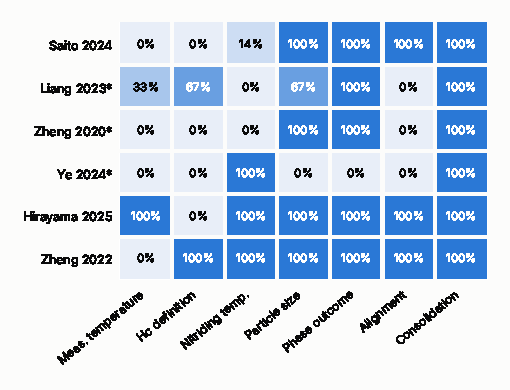
\includegraphics[width=\columnwidth]{fig2_completeness.pdf}
\caption{Reporting completeness by source: the share of each source's samples (rows) for which a comparison-relevant field (columns) is reported in the text available for extraction. Fields that do not apply (nitriding for samples made from commercial nitrided powder or not nitrided; consolidation for powders) count as reported. Asterisks mark sources read from the abstract only.}
\label{fig:complete}
\end{figure}

\subsection{Internal inconsistency}

One source reports the same quantity with two different values. Zheng \textit{et al.}~\cite{zheng2022} give a remanence of 10.19~kG in the abstract and 10.12~kG in the results and conclusions, a difference of 0.7\%. The database records the value supported by the results section and flags the discrepancy on the row. The difference is small, but a value-only extraction would have recorded whichever figure it encountered first, with no indication that the source disagrees with itself.

\section{Discussion}\label{sec:discussion}

\subsection{Implications for automated extraction}

The seed release shows why automated, value-only extraction is not enough for extrinsic magnet properties. The information that decides whether two values can be compared (measurement temperature, coercivity definition, sample form and basis) is missing or implicit for most values, even in recent open-access papers. An automated pipeline that does not record these fields must either discard the value or silently assume them. Both choices are invisible to the user. Recording the grade and its reasons makes the uncertainty explicit and auditable. The curation log adds a complementary lesson: the AI-assisted first draft transcribed every number correctly, but 3 of its evidence statements were paraphrases and 1 was attached to the wrong sentence. Verbatim evidence and an automated containment check are inexpensive safeguards against both.

Large text-mined databases and a curated, graded database are complementary. The former provide breadth and discovery~\cite{court2018,itani2025}; the latter provides a reference against which the accuracy of automated extraction can be measured for a specific materials family. A systematic comparison of OpenSmFe with text-mined entries for the same papers is planned for a later release.

\subsection{Recommended minimum reporting set}

The fields that most often prevented comparison suggest a minimum reporting set for experimental Sm--Fe--N magnet studies:
\begin{enumerate}\setlength{\itemsep}{0pt}
\item the measurement temperature of every hysteresis measurement;
\item the coercivity definition ($H_{cj}$ or $H_{cb}$) with units;
\item the instrument, maximum applied field, sample geometry and demagnetization correction, following established procedures for bulk magnets where they apply~\cite{iec604045,astma977};
\item the basis of every magnetization value and, for bulk or bonded magnets, the density;
\item the alloy route and the nitriding temperature, time, gas and pressure;
\item the phase analysis, including any $\alpha$-Fe fraction;
\item the particle-size distribution and the degree of alignment;
\item key values in a table rather than only in figures.
\end{enumerate}
None of these items is costly to report, and each one, if present, raises the comparability of the corresponding values.

\subsection{Limitations}\label{sec:limits}

Version 0.1 is a seed release of 6 papers. It demonstrates the method and does not describe the field; patterns in Fig.~\ref{fig:hc} reflect which papers were read, not which routes perform best. Only open-access papers are included, so the much larger subscription literature, including foundational work from the 1990s, is not yet represented, and the sample is skewed toward recent years. Of the 6 sources, 3 were read from the abstract only, and values appearing only in figures were not digitized. Values are recorded as published, without correction for demagnetization, density or sample shape. Compositions are nominal. Verification was recorded at the release level: the author verified every value against its source, but the confirmations that the verification log can hold row by row (the measurement temperature and coercivity definition from each paper's methods section) were not captured for v0.1. The grades are therefore conservative and can only rise as those confirmations are added.

\subsection{Outlook}

Version 1.0 will extend the release to the wider open-access literature, including U.S. Department of Energy public-access manuscripts and freely available Japanese journals in which much of the Sm--Fe--N literature appears. Values will be extracted from full-text PDFs and verified in batches, with row-level confirmations of temperature and coercivity definition. The planned composition--process--property maps are coercivity against particle size by route, remanence ratio against alignment, nitriding conditions against phase outcome, and Curie temperature against substitution. They will be built only from values whose grades allow the comparison.

\section{Conclusions}

OpenSmFe records Sm--Fe(--N) permanent-magnet properties together with the processing route, sample form and measurement conditions that give them meaning. It attaches a verbatim evidence sentence and an explicit comparability grade to every value. Applied to a seed release of 21 verified values, the approach shows that no value can yet be compared across sources without caveats, chiefly because measurement temperatures and coercivity definitions go unreported. It also shows that verbatim evidence and simple automated checks catch errors that value-only extraction would propagate. The schema, grading rules, workflow and data are openly available for reuse and extension, and the proposed reporting set offers a low-cost path to more comparable data in future studies.

\vspace{1.5ex}
\noindent\phead{Acknowledgments}This work received no specific funding.

\vspace{1ex}
\noindent\phead{AI assistance}The author used Claude (Anthropic; model Claude Opus 5.5) to search the literature, draft first-pass extractions, write the database code, figures and checks, and draft and revise the text. The author directed each step, verified every database value against its source, approved the scope and grading rules, checked the manuscript, and takes full responsibility for its content.

\vspace{1ex}
\noindent\phead{Data availability}The database, raw extraction tables, curation and verification logs, and the code that rebuilds every table, figure and number in this paper are openly available at https://github.com/johemeks/opensmfe (data CC BY 4.0, code MIT) and archived on Zenodo~\cite{opensmfe}.

\begin{thebibliography}{99}
\bibitem{gutfleisch2011} O. Gutfleisch, M. A. Willard, E. Br\"uck, C. H. Chen, S. G. Sankar, and J. P. Liu, Magnetic materials and devices for the 21st century: stronger, lighter, and more energy efficient, Adv. Mater. \textbf{23}, 821 (2011).
\bibitem{coey2020} J. M. D. Coey, Perspective and prospects for rare earth permanent magnets, Engineering \textbf{6}, 119 (2020).
\bibitem{doe2023} U.S. Department of Energy, \textit{Critical Materials Assessment} (U.S. Department of Energy, Washington, DC, 2023).
\bibitem{coeysun1990} J. M. D. Coey and H. Sun, Improved magnetic properties by treatment of iron-based rare earth intermetallic compounds in ammonia, J. Magn. Magn. Mater. \textbf{87}, L251 (1990).
\bibitem{xu2024} J. Xu, Y. Yi, B. Jia, H. Xue, G. Tian, Z. Ma, and Y. Hou, Composition and microstructural control of Sm$_2$Fe$_{17}$N$_3$ powders: a promising candidate for next-generation permanent magnets, J. Mater. Chem. C (2024), doi:10.1039/D4TC02797C.
\bibitem{saito2024} T. Saito, Production of Sm$_2$Fe$_{17}$N$_3$ bulk magnets, Inorganics \textbf{12}, 95 (2024).
\bibitem{zheng2022} J. Zheng, S. Yu, H. Huang, R. Li, W. Cai, H. Chen, J. Li, L. Qiao, Y. Ying, W. Li, J. Yu, and S. Che, Magnetic properties and microstructure of Ce--Cu--Al low melting alloy bonding Sm$_2$Fe$_{17}$N$_3$ magnet fabricated by the hot-pressing method, Magnetochemistry \textbf{8}, 149 (2022).
\bibitem{soda2016} R. Soda, K. Takagi, M. Jinno, W. Yamaguchi, and K. Ozaki, Anisotropic Sm$_2$Fe$_{17}$N$_3$ sintered magnets without coercivity deterioration, AIP Adv. \textbf{6}, 115108 (2016).
\bibitem{liang2023} D. Liang, W. Yang, X. Wang, Q. Xu, J. Han, S. Liu, C. Wang, H. Du, X. Zhu, T. Yuan, Z. Luo, and J. Yang, Study of the anisotropic Sm$_2$Fe$_{17}$N$_3$ powders with high performance, AIP Adv. \textbf{13}, 025104 (2023).
\bibitem{zheng2020} J. Zheng, S. Tian, K. Liu, W. Cai, Y. Tang, L. Qiao, Y. Ying, W. Li, J. Yu, Y. Liu, and S. Che, Preparation of submicron-sized Sm$_2$Fe$_{17}$N$_3$ fine powder by ultrasonic spray pyrolysis-hydrogen reduction (USP-HR) and subsequent reduction--diffusion process, AIP Adv. \textbf{10}, 055119 (2020).
\bibitem{okada2017} S. Okada, K. Suzuki, E. Node, K. Takagi, K. Ozaki, and Y. Enokido, Improvement of magnetization of submicron-sized high coercivity Sm$_2$Fe$_{17}$N$_3$ powder by using hydrothermally synthesized sintering-tolerant cubic hematite, AIP Adv. \textbf{7}, 056219 (2017).
\bibitem{hirayama2025} Y. Hirayama, J. Wang, M. Shigeta, S. Tsurumi, M. Sugimoto, Z. Liu, K. Takagi, and K. Ozaki, Nanosized anisotropic Sm--Fe--N particles with metastable TbCu$_7$-type structures prepared by an induction thermal plasma process, Nanomaterials \textbf{15}, 1045 (2025).
\bibitem{kronmuller2003} H. Kronm\"uller and M. F\"ahnle, \textit{Micromagnetism and the Microstructure of Ferromagnetic Solids} (Cambridge University Press, Cambridge, 2003).
\bibitem{iec604045} IEC 60404-5, \textit{Magnetic materials -- Part 5: Permanent magnet (magnetically hard) materials -- Methods of measurement of magnetic properties} (International Electrotechnical Commission, Geneva).
\bibitem{astma977} ASTM A977/A977M, \textit{Standard test method for magnetic properties of high-coercivity permanent magnet materials using hysteresigraphs} (ASTM International, West Conshohocken, PA).
\bibitem{coey2010} J. M. D. Coey, \textit{Magnetism and Magnetic Materials} (Cambridge University Press, Cambridge, 2010).
\bibitem{swain2016} M. C. Swain and J. M. Cole, ChemDataExtractor: a toolkit for automated extraction of chemical information from the scientific literature, J. Chem. Inf. Model. \textbf{56}, 1894 (2016).
\bibitem{mavracic2021} J. Mavra\v{c}i\'c, C. J. Court, T. Isazawa, S. R. Elliott, and J. M. Cole, ChemDataExtractor 2.0: autopopulated ontologies for materials science, J. Chem. Inf. Model. \textbf{61}, 4280 (2021).
\bibitem{court2018} C. J. Court and J. M. Cole, Auto-generated materials database of Curie and N\'eel temperatures via semi-supervised relationship extraction, Sci. Data \textbf{5}, 180111 (2018).
\bibitem{polak2024} M. P. Polak and D. Morgan, Extracting accurate materials data from research papers with conversational language models and prompt engineering, Nat. Commun. \textbf{15}, 1569 (2024).
\bibitem{itani2025} S. Itani, Y. Zhang, and J. Zang, The Northeast Materials Database for magnetic materials, Nat. Commun. \textbf{16} (2025), doi:10.1038/s41467-025-64458-z.
\bibitem{kim2017} E. Kim, K. Huang, A. Saunders, A. McCallum, G. Ceder, and E. Olivetti, Materials synthesis insights from scientific literature via text extraction and machine learning, Chem. Mater. \textbf{29}, 9436 (2017).
\bibitem{jain2013} A. Jain, S. P. Ong, G. Hautier, W. Chen, W. D. Richards, S. Dacek, S. Cholia, D. Gunter, D. Skinner, G. Ceder, and K. A. Persson, Commentary: The Materials Project: A materials genome approach to accelerating materials innovation, APL Mater. \textbf{1}, 011002 (2013).
\bibitem{wilkinson2016} M. D. Wilkinson \textit{et al.}, The FAIR Guiding Principles for scientific data management and stewardship, Sci. Data \textbf{3}, 160018 (2016).
\bibitem{doaj} Directory of Open Access Journals, https://doaj.org (accessed 8 October 2026).
\bibitem{opensmfe} J. C. Ejeka, OpenSmFe: an open, processing-aware database of samarium--iron(--nitrogen) permanent magnet properties, version 0.1.0, Zenodo (2026), doi:10.5281/zenodo.23248500; source code at https://github.com/johemeks/opensmfe.
\bibitem{ye2024} L. Ye, F. Wang, Y. Liu, H. Zhou, L. Liu, Y. Ding, Y. Sun, and A. Yan, New structural features and pinning-evolved coercivity mechanism: a potential route for developing high coercivities in anisotropic Sm--Fe--N material, J. Mater. Res. Technol. \textbf{30} (2024), doi:10.1016/j.jmrt.2024.03.040.
\end{thebibliography}
\end{document}
